\documentclass[cjk,slidestop,compress,mathserif,blue]{beamer}
%dvipdfm选项是关键,否则编译统统通不过
%beamer的颜色选项定义的是导航条和标题的颜色(即关键词structure的颜色)

%%%%%%%%%%%%%%%%仅限于XeTeX可使用的宏包%%%%%%%%%%%%%%%%%%%%%%%%%%%%
\usepackage{fontspec,xunicode,xltxtra,beamerthemesplit}
%\usepackage{beamerthemesplit}
\usepackage{xeCJK}
\setCJKmainfont[BoldFont=黑体, ItalicFont=楷体, BoldItalicFont=仿宋]{黑体}
%\setsansfont[Mapping=tex-text]{Adobe 黑体 Std}
%如果装了Adobe Acrobat,可在font.conf中配置Adobe字体的路径以使用其中文字体
%也可直接使用系统中的中文字体如SimSun,SimHei,微软雅黑 等
%原来beamer用的字体是sans family;注意Mapping的大小写,不能写错

%%%%%%%%   确定标题和导航条结构的框架     %%%%%%%%%%%%
\usepackage{beamerthemeshadow}                       %
%\usepackage{beamerthemeclassic}%导航条色与背景色一致%
%%%%%%%%%%%%%%%%%%%%%%%%%%%%%%%%%%%%%%%%%%%%%%%%%%%%%%
\setbeamerfont{roman title}{size={}}
%\usepackage{CJK} % CJK 中文支持                                  %
\usepackage{amsmath,amsthm,amsfonts,amssymb,bm}
\usepackage{mathrsfs}
\usepackage{xcolor}                                        %使用默认允许使用颜色
\usepackage{hyperref} 
\usepackage{graphicx}
\usepackage{subfigure}           %图片跨页

%\usepackage[numbers,sort&compress]{natbib} %紧密排列             %
\usepackage[sectionbib]{chapterbib}        %每章节单独参考文献   %
\usepackage{hypernat}                                                                         %
%\usepackage[dvipdfm,bookmarksopen=true,pdfstartview=FitH,CJKbookmarks]{hyperref}		%
\hypersetup{bookmarksnumbered,colorlinks,linkcolor=brown,citecolor=blue,urlcolor=red}         %
%参考文献含有超链接引用时需要下列宏包,注意与natbib有冲突        %
%\usepackage[dvipdfm]{hyperref}                                  %
%\usepackage{hypernat}                                           %
\newcommand{\upcite}[1]{\hspace{0ex}\textsuperscript{\cite{#1}}} %

%\useoutertheme{smoothbars}
\useinnertheme[shadow=true]{rounded}
\usetheme{Berkeley}                                          %主题式样
%\usetheme{Luebeck}

\usecolortheme{lily}                                        %颜色主题式样

\usefonttheme{professionalfonts}                           %字体主题样式宏包

%\beamertemplatetransparentcoveredhigh                      %使所有被隐藏的文本高度透明
\beamertemplatetransparentcovereddynamicmedium             %使所有被隐藏的文本完全透明,动态,动态的范围很小
\mode<presentation>
%\beamersetaveragebackground{gray}                          %设置背景颜色(单一色) 
\beamertemplateshadingbackground{green!10}{red!5}         %设置背景颜色(渐变色)

%在指定位置精确放置logo
\usepackage{tikz}
\usepackage{beamerfoils}
\usepackage{pgf}
\logo{\pgfputat{\pgfxy(11.68,0.15)}{
\includegraphics[height=1.01cm,viewport=0 0 140 120,clip]{Figures/BCC_logo-1.png}}\pgfputat{\pgfxy(10.502,-0.218)}{
\includegraphics[height=0.369cm,viewport=140 0 540 120,clip]{Figures/BCC_logo-1.png}}}
%\logo{\pgfputat{\pgfxy(11.68,0.15)}{
\includegraphics[height=0.95cm,viewport=0 0 510 360,clip]{Figures/Logo_Gainstrong.png}}\pgfputat{\pgfxy(10.333,-0.195)}{
\includegraphics[height=0.35cm,viewport=530 70 1100 218,clip]{Figures/Logo_Gainstrong.png}}}
%\MyLogo{
%	\pgfputat{\pgfxy(-50,-50)}{\pgfbox[right,base]{
\includegraphics[height=1cm]{Figures/BCC_logo-1.png}}}

%logo作为背景放置
%\setbeamertemplate{background}{
%	\pgfputat{\pgfxy(6.5,-0.5)}{\pgfbox[left,top]{\pgfimage[height=1.1cm]{Figures/BCC_logo-1.png}}}}

%\logo{}									%不显示logo

\begin{document}
%\begin{CJK*}{GBK}{song}
%\begin{CJK*}{GBK}{kai}
%beamer下不能用\songyi、\zihao等命令!
%\graphicspath{Figures/}

%-------------------------------PPT Title-------------------------------------
\title{KKR方法与LMTO方法概述}
%-----------------------------------------------------------------------------

%----------------------------Author & Date------------------------------------
\author{北京市计算中心\;云平台\:姜骏}
\date{\textrm{2016.11.02}}
%\date{2013.09.10}
\frame{\titlepage}
%-----------------------------------------------------------------------------

%------------------------------------------------------------------------------列出全文 outline ---------------------------------------------------------------------------------
\section*{}
\frame[allowframebreaks]
{
  \frametitle{Outline}
%  \frametitle{\textcolor{mycolor}{\secname}}
  \tableofcontents%[current,currentsection,currentsubsection]
}
%在每个section之前列出全部Outline
%类似的在每个subsection之前列出全部Outline是\AtBeginSubsection[]
\AtBeginSection[]
{
  \frame<handout:0>
  {
    \frametitle{Outline}
%全部Outline中,本部分加亮
    \tableofcontents[current,currentsection]
  }
}

%------------------------------------------------------------------------------PPT main Body------------------------------------------------------------------------------------
\small
\section{KKR方法}
\frame
{
	\frametitle{独立粒子的\textrm{Green's function}}
\textrm{KKR}方法最初是由\textrm{Korringa}\upcite{PA13-392_1947},~\textrm{Kohn}和\textrm{Rostoker}\upcite{PR94-1111_1954}根据多重散射理论\textrm{(Multi-scattering theory, MST)}提出的,本质上这是一种\textrm{Green's function}方法

利用\textrm{Green's function},可以将\textrm{Schr\"odinger}方程变成齐次积分方程的形式:
\begin{displaymath}
	\Psi_{\vec k}(\vec k)=\int_{\Omega_0}\tilde G_0(\varepsilon;\vec r-\vec r\,^{\prime})V(\vec r\,^{\prime})\Psi_{\vec k}(\vec r\,^{\prime})\mathrm{d}\vec r\,^{\prime}
\end{displaymath}
这里$\Omega_0$是重复单元体积\\$\tilde G_0$是满足\textrm{Bl\"och}周期条件的独立粒子的\textrm{Green's function},%可以写成
%\begin{displaymath}
%	\begin{aligned}
%		\tilde G_{\vec k}(\vec r-\vec r\,^{\prime};E)=&-\dfrac1{4\pi}\sum_n\mathrm{e}^{\mathrm{i}\vec k\cdot\vec R_n}\dfrac{\cos(q_0|\vec r-\vec r\,^{\prime-\vec R_n}|)}{|\vec r-\vec r\,^{\prime}-\vec R_n|}\\
%		=&-\Omega_0^{-1}\sum_n\dfrac{\exp[\mathrm{i}(\vec k+\vec G_n)\cdot(\vec r-\vec r\,^{\prime})]}{|\vec k+\vec G_n|^2-E}
%	\end{aligned}
%\end{displaymath}
%这里$q_0=\sqrt E$,$\vec G_n$是到空间格矢,$\vec R_n$是晶格平移矢量。
满足%\textrm{Dyson}方程
\begin{displaymath}
	\left[-\dfrac12\nabla^2-(\varepsilon-V_0)\right]\tilde G_0(\varepsilon;\vec r-\vec r\,^{\prime})=\delta(\vec r-\vec r\,^{\prime})
\end{displaymath}
这里势能$V_0$是常数
}

\frame{
	\frametitle{\textrm{KKR}方法的本征态表示}
	根据\textrm{Green's function~}传播子理论
	\begin{itemize}
		\item \textrm{MT}球条件下波函数可以表示为
			\begin{displaymath}
				\psi_{\vec k}(\vec r)=-\int\mathrm{d}\vec r\,^{\prime}\tilde G_0(\varepsilon_{\vec k}^n,|\vec r-\vec r\,^{\prime}|)V(\vec r\,^{\prime})\psi_{\vec k}(\vec r\,^{\prime})
			\end{displaymath}
		\item \textrm{Green's function~}分电荷密度表示为
			\begin{displaymath}
				\begin{aligned}
					n_L(\varepsilon,\vec k)=&-\dfrac1{\pi}\Im\tilde G_{LL^{\prime}}(\varepsilon+\mathrm{i}\delta,\vec k)\quad\mbox{倒空间表示}\\
					n_L(\varepsilon,\vec R)=&-\dfrac1{\pi}\Im\tilde G_{LL^{\prime}}(\varepsilon+\mathrm{i}\delta,\vec R)\quad\mbox{正空间表示}
				\end{aligned}
			\end{displaymath}
		\item 能量本征态的表示
			\begin{displaymath}
				\sum_i\varepsilon_i=\dfrac1{\pi}\int_{E_{\mathrm{F}}}^{\infty}\mathrm{d}\varepsilon\,\varepsilon\Im\tilde G_{LL^{\prime}}(\varepsilon+\mathrm{i}\delta,0)
			\end{displaymath}
	\end{itemize}
}

\frame
{
	\frametitle{球形势的单重散射}
\begin{figure}[h!]
\centering
\vspace*{-0.26in}
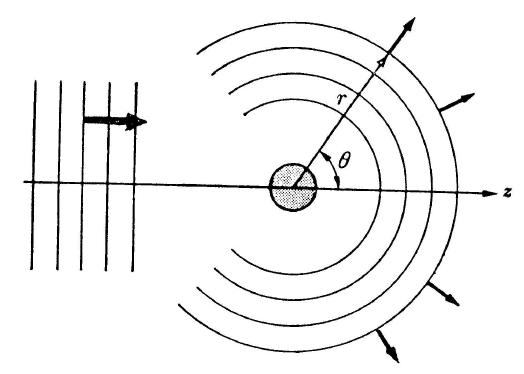
\includegraphics[height=1.60in,width=2.20in,viewport=0 0 400 300,clip]{Figures/Pseudo-scatter.jpg}
\caption{\small \textrm{Schematic illustration of scattering of a plane wave by a spherical potential.}}%(与文献\cite{EPJB33-47_2003}图1对比)
\label{Pseudo-scatter}
\end{figure}
入射波为自由电子(平面波)时,经过球对称势的散射,出射波函数形式为
$$\psi_L(\vec r)=\mathrm{i}^l\psi_l(r)Y_L(\hat{\vec }r)=\mathrm{i}^lr^{-1}\phi_l(r)Y_L(\hat{\vec }r)$$
}

\frame
{
	\frametitle{\textrm{MT}球势与散射}
	在\textrm{MT}球形势近似下,离子实对电子的散射振幅$t_l(\varepsilon)$服从角动量守恒,可以用相移$\eta_l(\varepsilon)$表示
	$$t_l(\varepsilon)=\dfrac{\mathrm{i}}{2q_0}\big[\mathrm{e}^{\mathrm{i}2\eta_l(\varepsilon)}-1\big]=-\dfrac1{q_0}\mathrm{e}^{\mathrm{i}\eta_l(\varepsilon)}\sin(\eta_l(\varepsilon))$$
	这里$\varepsilon=q_0^2$

	同时,在\textrm{MT}球外,散射波函数用相移表示为
	$$\psi_l^{>}(\varepsilon,r)=C_l[j_l(q_0r)-\tan(\eta_l(\varepsilon))n_l(q_0r)]$$
	\textcolor{blue}{独立粒子\textrm{Green's function~}$\tilde G_0(\varepsilon;\vec r-\vec r\,^{\prime})$描述的是具有能量$\varepsilon$的独立粒子由点$\vec r$向$\vec r\,^{\prime}$的传播}\\
	\textrm{MT}势对入射平面波单重散射的\textrm{Green's function~}$\tilde G_0(\varepsilon,\vec r-\vec r\,^{\prime})$%满足方程
%	\begin{displaymath}
%		\left[-\dfrac{\hbar^2}{2m_e}\nabla_r^2-(\varepsilon-V_0)\right]\tilde G_0(\varepsilon,\vec r-\vec r\,^{\prime})=\delta(\vec r-\vec r\,^{\prime})
%	\end{displaymath}
	具有解析形式
	$$\tilde G_0(\varepsilon,|\vec r-\vec r\,^{\prime}|)=\dfrac{2m_e}{\hbar^2}\dfrac1{4\pi}\dfrac{\cos(q_0|\vec r-\vec r\,^{\prime}|)}{|\vec r-\vec r\,^{\prime}|}$$
	$\tilde G_0$只与结构和能量$\varepsilon$有关%\\\textcolor{red}{$\mathbf{t}$包含\textrm{MT}球对电子单重散射的全部信息}

%	用相移$\eta_l(\varepsilon)$表示电子结构和\textrm{Green's function}最显著的优点:\\一般$l$~取值只需要$l\leqslant3$
}

\frame
{
	\frametitle{多重散射与\textrm{Green's function}}
\begin{figure}[h!]
	\vspace{-40pt}
\centering
%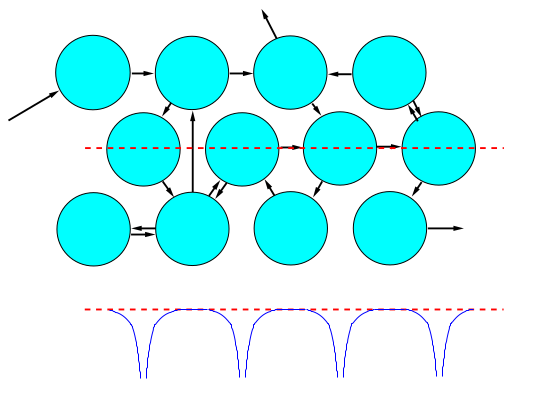
\includegraphics[height=1.80in,width=1.95in,viewport=5 0 515 495,clip]{Figures/multiple-scattering_theory.png}
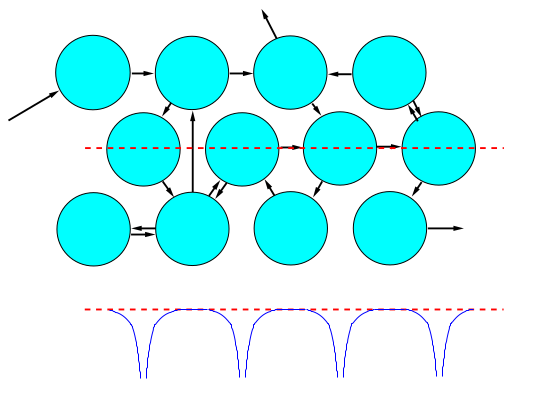
\includegraphics[height=1.70in,width=1.82in,viewport=5 0 515 495,clip]{Figures/multiple-scattering_theory.png}
\caption{\small \textrm{Central idea of multiple scattering theory:~ decomposition of electronic motion into scattering at atomic sites and free-electron like propagation in between. The bottom of the figure gives a sketch for the potential along the dashed line.}}
\label{Multi-scattering}
\end{figure}
\textcolor{blue}{多重散射:~}入射波是\textcolor{red}{所有来自其他散射中心的出射波叠加}
			\begin{displaymath}
				\begin{aligned}
					\tilde G=&\tilde G_0+G_0\mathbf{t}\tilde G_0+G_0\mathbf{t}\tilde G_0\mathbf{t}\tilde G_0+\cdots\\
					=&\tilde G_0+\tilde G_0\mathbf{t}\tilde G \Longrightarrow \tilde G=(\tilde G_0^{-1}-\mathbf{t})^{-1}
%					\tilde G=&(\tilde G_0^{-1}-\mathbf{t})^{-1}
				\end{aligned}
			\end{displaymath}
}

\frame
{
	\frametitle{\textrm{MT}势的\textrm{Green's function}}
	引入散射矩阵$\mathbf{T}$描述体系对电子的散射,其矩阵元$\mathbf{t}$表示\textrm{MT}球内散射中心的各种影响\\
			\begin{displaymath}
				\begin{aligned}
					\mathbf{T}=&\mathbf{t}+\mathbf{t}\tilde G_0\mathbf{t}+\mathbf{t}\tilde G_0\mathbf{t}\tilde G_0\mathbf{t}+\cdots\\
					=&\mathbf{t}+\mathbf{t}\tilde G_0(\mathbf{t}+\mathbf{t}\tilde G_0\mathbf{t}+\cdots \\ 
					=&\mathbf{t}+\mathbf{t}\tilde G_0\mathbf{T}\Longrightarrow\\
					\mathbf{T}=&(\mathbf{t}^{-1}-\tilde G_0)^{-1}
				\end{aligned}
			\end{displaymath}
			经过多重散射,\textrm{Green's function}函数可以表示为$$\tilde G=\tilde G_0+\tilde G_0\mathbf{T}\tilde G_0$$
			一般地,根据散射理论,\textrm{Green's function}可以用散射振幅$t_l(\varepsilon, \vec R)$与\textrm{MT}球芯位置$\vec R$(结构参数)表示
\begin{displaymath}
	[G_{LL^{\prime}}(\varepsilon;\vec R,\vec R\,^{\prime})]^{-1}=\big[[B_{L,L^{\prime}}(\varepsilon;\vec R-\vec R\,^{\prime})]^{-1}-t_l(\varepsilon,\vec R)\delta_{\vec R,\vec R^{\prime}}\delta_{L,L^{\prime}}\big]
\end{displaymath}
}

\frame
{
	\frametitle{\textrm{MT}势的\textrm{Green's function}}
	其中$B_{LL^{\prime}}$称为\textcolor{blue}{\textrm{KKR}结构矩阵}
	\begin{displaymath}
		\tilde B(\varepsilon;\vec R-\vec R\,^{\prime})=%\sum_{LL^{\prime}}A_{LL^{\prime}}j_l(q_0r)j_{l^{\prime}}(q_0r\,^{\prime})\times Y_L(\hat r)Y_{L^{\prime}}(\hat{\vec r}\,^{\prime})
		-4\pi q_0\sum_{L^{\prime\prime}}\mathrm{i}^{l^{\prime\prime}}C_{L^{\prime}L^{\prime\prime}}^Ln_{l^{\prime\prime}}(q|\vec R-\vec R\,^{\prime}|)Y_{L^{\prime}}^{\ast}(\widehat{\vec R-\vec R\,^{\prime}})
	\end{displaymath}
%	这里$A_{LL^{\prime}}$称为\textrm{KKR}结构常数,满足周期边界条件。
%	\begin{displaymath}
%		A_{LL^{\prime}}(\vec r,\varepsilon)=4\pi q_0\sum_{\vec R_n\neq 0}\mathrm{e}^{\mathrm{i}\vec k\cdot\vec R_n}\sum_{l^{\prime\prime}}\mathrm{i}^{l^{\prime}-l-l^{\prime\prime}}n_{l^{\prime\prime}}(q_0R_n)Y_{L^{\prime\prime}}^{\ast}(\hat{\vec R}_n)C_{LL^{\prime}L^{\prime\prime}}
%	\end{displaymath}

	$C_{L^{\prime}L^{\prime\prime}}^L$是\textrm{Gaunt}系数
	\begin{displaymath}
		C_{L^{\prime}L^{\prime\prime}}^L=\int Y_L(\hat{\vec r})Y_{L^{\prime}}^{\ast}(\hat{\vec r})Y_{L^{\prime\prime}}(\hat{\vec r})\mathrm{d}\Omega_0
	\end{displaymath}
	\textrm{Green's function~}的单中心散射和多重散射部分分别用径向函数和球谐函数展开后,要求径向函数在全部\textrm{MT}球面上连续,可有
	\begin{displaymath}
		\det\big[t_l^{-1}(\varepsilon,\vec R)\delta_{\vec R,\vec R^{\prime}}\delta_{L,L^{\prime}}-B_{L,L^{\prime}}(\varepsilon;\vec R-\vec R\,^{\prime})\big]=0
	\end{displaymath}
	这就是\textrm{Wronskian}关系(\textrm{KKR}方程)\\
	\textcolor{red}{由此确定的能量$\varepsilon$,即与体系的本征值对应}
}

\frame
{
	\frametitle{\textrm{MT}势的\textrm{Green's function}}
	通过\textrm{Green's function},\textrm{MT}球对入射波的散射可以分解为两部分
\begin{displaymath}
	\begin{aligned}
		G(\varepsilon;\vec r+\vec R^n,\vec r\,^{\prime}+\vec R\,^{n^\prime})=&\underbrace{\delta_{nn^{\prime}}q_0\sum_LH_L^n(\varepsilon;\vec r_>)R_L^n(\varepsilon;\vec r_<)}\\
		&\mbox{\qquad\textcolor{red}{单中心散射部分贡献}}\\
		&+\underbrace{\sum_{LL^{\prime}}R_L^n(\varepsilon;\vec r)B_{LL^{\prime}}^{nn^{\prime}}(\varepsilon)R_{L^{\prime}}^{n^{\prime}}(\varepsilon;\vec r)}\\
		&\mbox{\quad\qquad\textcolor{red}{多重散射部分贡献}}
	\end{aligned}
\end{displaymath}
这里$\vec r$和$\vec r\,^{\prime}$分别对应\textrm{MT}球$\vec R^n$和$\vec R\,^{n^\prime}$;$\vec r_<$和$\vec r_>$分别是$\vec r$和$\vec r\,^{\prime}$小的和大的\\
\begin{displaymath}
	\begin{aligned}
		\textcolor{blue}{r^l}\xleftarrow{r\rightarrow0}R_L^n(\varepsilon;\vec r)=&R_l^n(\varepsilon;\vec r)Y_L(\hat{\vec r})\rightarrow\textcolor{blue}{j_l(q_0r)Y_L(\hat{\vec r})}\\
		\textcolor{blue}{r^{l+1}}\xleftarrow{r\rightarrow0}H_L^n(\varepsilon;\vec r)=&H_l^n(\varepsilon;\vec r)Y_L(\hat{\vec r})\rightarrow\textcolor{blue}{h_l(q_0r)Y_L(\hat{\vec r})}
	\end{aligned}
\end{displaymath}
}

\frame
{
	\frametitle{\textrm{KKR}方法的特点}
%	当原胞内使用\textrm{MT}势满足\textrm{MT}球内对称势$V(\vec r)$,间隙区的势为$V=0$时,满足\textrm{Dyson}方程的\textrm{Green's function~}$\tilde G_{\vec k}$可以用球谐函数$Y_L(\hat{\vec r})$,球\textrm{Bessel}函数$j_l(x)$和\textrm{Neumann}函数$n_l(x)$展开表示,并写成两项之和
%	在实际应用中,用\textrm{Green's function}求解\textrm{MT}势下的多重散射问题,选择
% 其中$G_0$仅与结构和能量$\varepsilon$有关,$t$包含了\textrm{MT}势在球内的各种影响,由此可得
%	\begin{displaymath}
%		\tilde G_0(\varepsilon;\vec r-\vec r\,^{\prime})=\sum_{L,L^{\prime}}\mathrm{i}^lj_l(q_0r)Y_L(\hat{\vec r})B_{LL^{\prime}}(-\mathrm{i})^{l^{\prime}}j_l^{\prime}(q_0r^{\prime})Y_{L^{\prime}}(\hat{\vec r}\,^{\prime})
%	\end{displaymath}
%	\begin{displaymath}
%		\tilde G_{\vec k}(\varepsilon;\vec r-\vec r\,^{\prime})=\tilde G_0(\varepsilon;\vec r-\vec r\,^{\prime})+B_{\vec k}(\varepsilon;\vec r-\vec r\,^{\prime})
%	\end{displaymath}
%	其中$\tilde G_0(\varepsilon;\vec r-\vec r\,^{\prime})$可以选\textrm{Helmholtz}方程$$(\nabla^2+q_0^2)\tilde G_0(\varepsilon;\vec r-\vec r\,^{\prime})=\delta(\vec r-\vec r\,^{\prime})$$的实数解
%	\begin{displaymath}
%		\begin{aligned}
%			\tilde G_0(\varepsilon;\vec r-\vec r\,^{\prime})=&-\dfrac1{4\pi}\dfrac{\cos(q_0|\vec r-\vec r\,^{\prime}|)}{|\vec r-\vec r\,^{\prime}|}\\
%			=&q_0\sum_Lj_l(q_0r)n_l(q_0r)\times Y_L(\hat r)Y_L^{\ast}(\hat{\vec r}\,^{\prime})\quad r<r\,^{\prime}
%		\end{aligned}
%	\end{displaymath}
%这里$q_0=\sqrt\varepsilon$
	实际应用中,\textrm{Green's function}的球谐函数展开,在\textrm{MT}球面上收敛非常慢,需要很大的$l_{\max}$\\根据多重散射理论,\textrm{Green's function}影响在\textrm{MT}球内,势函数$v_l(\vec r)$展开收敛快速,因此结构矩阵可用\textrm{Dyson}方程表示
	$$B_{LL^{\prime}}^{nn^{\prime}}(\varepsilon)=g_{LL^{\prime}}^{nn^{\prime}}(\varepsilon)+\sum_{n^{\prime\prime}L^{\prime\prime}}g_{LL^{\prime\prime}}^{nn^{\prime\prime}}t_{l^{\prime\prime}}^{n^{\prime\prime}}B_{LL^{\prime\prime}}^{nn^{\prime\prime}}$$
	其中由势$v^(r)$确定的$t_l^n$
	$$t_l^n(\varepsilon)=\int_0^{R^n}\mathrm{d}r\,r^2j_l(q_0r)v^n(r)R_l^n(\varepsilon;r)$$
	$g_{LL^{\prime}}^{nn^{\prime}}$是自由电子的结构矩阵,具有解析形式

	\textcolor{blue}{\textrm{KKR-Green's function}方法的特点}
	\begin{itemize}
		\item \textcolor{red}{基函数是优化的最小基组,计算基本不随基组增减影响}
		\item \textcolor{red}{不同计算体系,所选基组对经验的依赖很大}
	\end{itemize}
}

\frame
{
	\frametitle{周期条件下\textrm{MT}势的\textrm{Green's function}}
周期条件下结构常数$B_{LL^{\prime}}(\varepsilon,\vec k)$定义为
\begin{displaymath}
	B_{LL^{\prime}}(\varepsilon,\vec k)=\sum_{\vec T}B_{LL^{\prime}}(\varepsilon,\vec T)\mathrm{e}^{-\mathrm{i}\vec k\cdot\vec T}
\end{displaymath}
由此得到方程
\begin{displaymath}
	\det[t_l^{-1}(\varepsilon)\delta_{LL^{\prime}}-B_{LL^{\prime}}(\varepsilon,\vec k)]=0
\end{displaymath}
的解是能量$\varepsilon_{\vec k}$

用相移表示$t_l$,可以得到\textrm{KKR}方程
\begin{displaymath}
	\sum_{L^{\prime}}[B_{LL^{\prime}}(\varepsilon_{\vec k},\vec k)+q_0\cot(\eta_l(\varepsilon_k))\delta_{LL^{\prime}}]a_L^{\prime}(\vec k)=0
\end{displaymath}
如果一个原胞中含有原子数$\alpha=1,2,3,\cdots,N$
\begin{displaymath}
	\sum_{\beta=1}^N\sum_{L^{\prime}}[B_{LL^{\prime}}(\tau_{\alpha}-\tau_{\beta},\varepsilon_{\vec k},\vec k)+q_0\cot(\eta_{l\beta}(\varepsilon_k))\delta_{LL^{\prime}}\delta_{\alpha\beta}]a_{L^{\prime}\beta}(\vec k)=0
\end{displaymath}
}

\section{MTO与LMTO方法}
\frame
{
\frametitle{\textrm{MTO}方法}
\textrm{MTO (Muffin-tin Orbial)}方法是\textrm{Andersen}于\textrm{1971}年提出的局域缀加基函数方案\upcite{Andersen_Book}。
%\textrm{MTO}的
\textcolor{blue}{目的:~用最小基组方法解析电子结构}

\textrm{MTO}的特点
\begin{itemize}
	\item \textcolor{red}{物理图像}:~和\textrm{APW}方法类似,要求基函数在\textrm{MT}球内、外分区域表示,并且在球面上连续
	\item \textcolor{red}{数学形式}:~基函数是与\textrm{KKR}方法相似的最小优化基组
		\begin{enumerate}
			\item \textrm{MT}球内基函数是\textrm{MT}球的散射分波 
				$$\psi_l(\varepsilon,\vec r)=\mathrm{i}^lr^{-1}\phi_l(\varepsilon,\vec r)Y_L(\hat{\vec r})$$
			\item \textrm{MT}根据散射理论,\textrm{MT}球外基函数形如$$\psi_l(\varepsilon,\vec r)\propto j_l(q_0r)-\tan(\eta_l(\varepsilon))n_l(q_0r)$$
			\item 当$\varepsilon<0$,\textrm{Neumann}函数$n_l$可用\textrm{Hankel}函数$h_l=j_l+\mathrm{i}\eta_l$替换,由此\textrm{MT}球外基函数形式为$$\psi_l(\varepsilon,\vec r)\propto\mathrm{i}^{-l}\mathrm{e}^{-|q_0|r}/|q_0|r$$
				\textcolor{red}{只有$\varepsilon$对应体系本征值时,函数在\textrm{MT}球面上连续}
		\end{enumerate}
\end{itemize}

%		特别地,当能量$\varepsilon<0$,\textrm{Neumannn}函数$n_l$用\textrm{Hankel}函数$h_l$代替$$h_l^{(1)}=j_l+\mathrm{i}\eta_l$$渐近形式为$\frac{\mathrm{i}^{-l}\mathrm{e}^{-|q_0|r}}{|q_0|r}$\\
%		此时球\textrm{Bessel}是非约束的,这样的轨道不适合做基函数:~因为当能量$\varepsilon<0$,只有当能量$\varepsilon=\varepsilon_{\vec k}$,球\textrm{Bessel}函数的系数为0,基函数才可能是正交归一
}

\frame
{
\frametitle{\textrm{MTO}方法的基函数}
%\textcolor{red}{“展开定理”可用来判断具有解析形式的函数是否适宜作为基函数:~}
%以$R$为中心的函数用临近位置的基函数展开
%\begin{displaymath}
%	\chi_{\alpha}(\vec r-\vec R)=\sum_{\alpha^{\prime}}B_{\alpha\alpha^{\prime}}(\vec R,\vec R^{\prime})\chi_{\alpha^{\prime}}(r-R^{\prime})
%\end{displaymath}
%该定理对于积分非常有用:~
%
上述单重散射模型给出的\textrm{MTO}函数不适宜作为\textrm{MTO~}基函数,\textrm{Andersen~}根据多重散射理论重构了基函数
		\begin{displaymath}
			\hspace*{-10pt}\chi_L^{\mathrm{MTO}}(\varepsilon,q_0,\vec r)=\mathrm{i}^lY_L(\hat{\vec r})\left\{
			\begin{aligned}
				&\psi_l(\varepsilon,r)+q_0\cot(\eta_l(\varepsilon))j_l(q_0r)&\quad r\leqslant S\\
				&q_0n_l(q_0r)&\quad r>S
			\end{aligned}\right.
		\end{displaymath}
		\textrm{Andersen~}构造的\textrm{MTO}基函数的特点
		\begin{itemize}
			\item \textcolor{blue}{\textrm{MT}球外部分函数形式简单}
			\item \textcolor{red}{\textrm{MTO}内的函数包含来自其他散射函数的贡献($j_l$部分)}
		\end{itemize}
		根据多重散射理论,球面波函数延伸到\textrm{MT}球外部分,可用球\textrm{Bessel}函数展开表示
		\begin{displaymath}
			n_L(q_0,\vec r-\vec R)=4\pi\sum_{L^{\prime}L^{\prime\prime}}C_{L^{\prime}L^{\prime\prime}}^Ln_{L^{\prime\prime}}^{\ast}(q_0,\vec R-\vec R\,^{\prime})j_{L^{\prime}}(q_0,\vec r-\vec R\,^{\prime})
		\end{displaymath}
		其中$C_{L^{\prime}L^{\prime\prime}}^L$是\textrm{Gaunt}系数

%		只有当能量参数$\varepsilon$对应体系的本征值时,用\textrm{MTO}基函数展开的波函数对应于体系本征态

		这里参数(衰减常数)$q_0$由$q_0^2=\varepsilon-V_0$确定
}

\frame
{
	\frametitle{\textrm{MTO}方法的基函数}
\begin{figure}[h!]
\centering
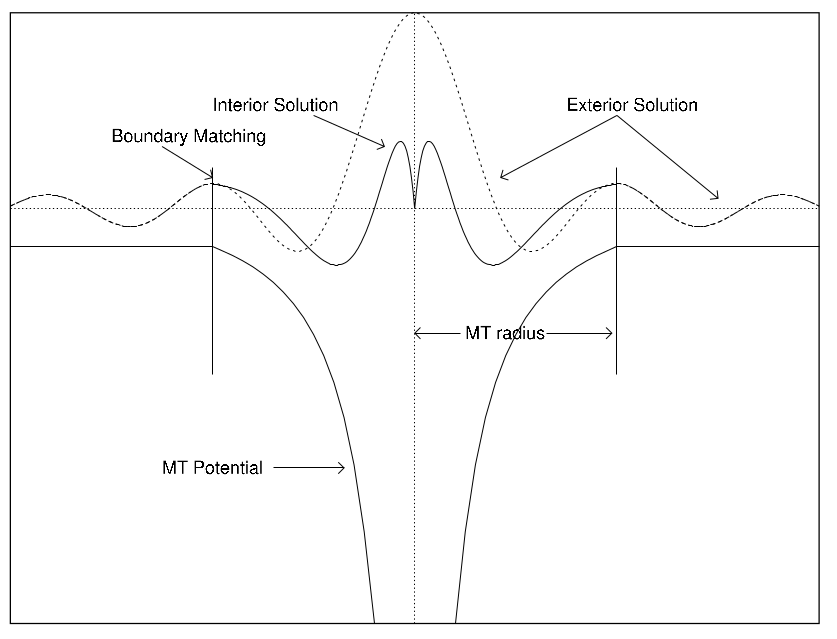
\includegraphics[height=1.70in,width=2.15in,viewport=0 0 845 635,clip]{Figures/MTO-envelope-1.png}
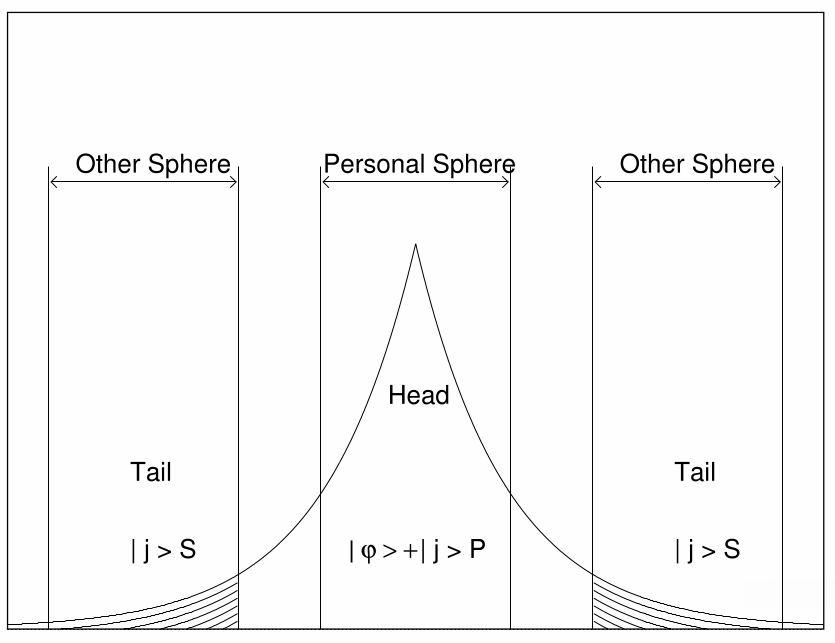
\includegraphics[height=1.70in,width=2.15in,viewport=0 0 885 635,clip]{Figures/MTO-envelope-2.png}
\caption{\small \textrm{The radial function of MTO expressed in different region.}}%(与文献\cite{EPJB33-47_2003}图1对比)
\label{MTO-envelope}
\end{figure}
}

\frame
{
	\frametitle{\textrm{MTO-ASA}}
\begin{figure}[h!]
	\vspace{-18pt}
\centering
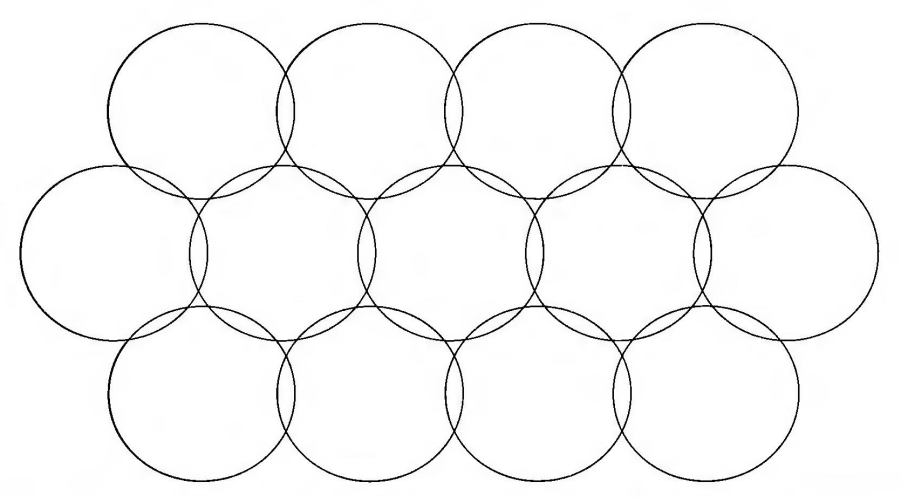
\includegraphics[height=1.20in,width=2.42in,viewport=5 0 1005 495,clip]{Figures/Atomic_sphere-appro.png}
\caption{\small \textrm{Atomic sphere approximation (ASA) in which the MT spheres are chosen to have the same volume as the Wigner-Seitz cell, which leads to overlapping spheres.}}
\label{Atomic_sphere-appro}
\end{figure}
当$q_0=0$时,构成最简单的\textrm{MTO}基函数
		\begin{displaymath}
			\hspace*{-12pt}\chi_L^{\mathrm{MTO}}(\varepsilon,0,\vec r)=\mathrm{i}^lY_L(\hat{\vec r})\psi_l(\varepsilon,S)\left\{
			\begin{aligned}
				&\dfrac{\psi_l(\varepsilon,r)}{\psi_l(\varepsilon,S)}-\dfrac{D_l(\varepsilon)+l+1}{2l+l}\left(\dfrac rS\right)^l&\, r\leqslant S\\
				&+\dfrac{l-D_l(\varepsilon)}{2l+1}\left(\dfrac Sr\right)^{l+1}&\, r>S
			\end{aligned}\right.
		\end{displaymath}
}

\frame
{
	\frametitle{正则能带基函数}
	$D_l(\varepsilon)$是径向分波$\psi_l(\varepsilon,r)$在球面$r=S$位置的对数导数
%	\begin{displaymath}
%		\hspace*{-15pt}\begin{aligned}
%			&\left[\dfrac S{|\vec r-\vec R|}\right]^{l+1}\mathrm{i}^lY_L(\widehat{\vec r-\vec R})\\
%				=&4\pi\sum_{L^{\prime}}\bigg[\dfrac rS\bigg]^{l^{\prime}}\mathrm{i}^{l^{\prime}}Y_{L^{\prime}}(\hat{\vec r})\left\{\dfrac{(2l^{\prime\prime}-1)!!}{(2l-1)!!(2l^{\prime}+1)!!}C_{L^{\prime}L^{\prime\prime}}^L\bigg[\dfrac S{|\vec R|}\bigg]^{l^{\prime\prime}+1}\mathrm{i}^{-l^{\prime\prime}}Y_{L^{\prime\prime}}^{\ast}(\hat{\vec R})\right\}
%		\end{aligned}
%	\end{displaymath}

	\textcolor{blue}{考虑平移周期性},
$$\chi_{L,\vec k}^{\mathrm{MTO}}(\varepsilon,0,\vec r)=\sum_{\vec T}\mathrm{e}^{\mathrm{i}\vec k\cdot\vec R}\chi_L^{\mathrm{MTO}}(\varepsilon,0,\vec r)$$
\textcolor{blue}{\textrm{MT}球内的\textrm{MTO-ASA}的基函数为}
\begin{displaymath}
	\begin{aligned}
		\chi_{L,\vec k}^{\mathrm{MTO}}(\varepsilon,0,\vec r)=&\underline{\textcolor{red}{\psi_l(\varepsilon,r)\mathrm{i}^lY_L(\hat{\vec r})}}-\dfrac{D_l(\varepsilon)+l+1}{2l+l}\psi_l(\varepsilon,S)\left(\dfrac rS\right)^l\mathrm{i}^lY_L(\hat{\vec r})\\
		&+\dfrac{l-D_l(\varepsilon)}{2l+1}\psi_l(\varepsilon,S)\sum_{L^{\prime}}\left(\dfrac rS\right)^{l^{\prime}}Y_{L^{\prime}}(\hat{\vec r})S_{LL^{\prime}}(\vec k)
	\end{aligned}
\end{displaymath}
其中
\begin{displaymath}
	\begin{aligned}
		S_{LL^{\prime}}(\vec k)=&2(2l+1)\dfrac{[D_l(\varepsilon)+l+1]}{[D_l(\varepsilon)-1]}\\
		=&g_{l^{\prime}m^{\prime},lm}\sum_{\vec T}\mathrm{e}^{\mathrm{i}\vec k\cdot\vec T}\bigg[\dfrac S{|\vec T|}\bigg]^{l^{\prime\prime}+1}\big[\sqrt{4\pi}\mathrm{i}^{l^{\prime\prime}}Y_{L^{\prime\prime}}(\hat{\vec T})\big]^{\ast}
	\end{aligned}
\end{displaymath}
}

\frame
{
	\frametitle{正则能带}
	\textcolor{red}{$\psi_l(\varepsilon,r)\mathrm{i}^lY_L(\hat{\vec r})$是\textrm{MT}球内满足原子分波函数的形式}
	\begin{itemize}
		\item \textcolor{blue}{在\textrm{MT}球内来自其他原子尾部贡献部分}$$\dfrac{l-D_l(\varepsilon)}{2l+1}\psi_l(\varepsilon,S)\sum_{L^{\prime}}\left(\dfrac rS\right)^{l^{\prime}}Y_{L^{\prime}}(\hat{\vec r})S_{LL^{\prime}}(\vec k)$$
		\item \textcolor{blue}{在\textrm{MT}球内非物理贡献部分}$$\dfrac{D_l(\varepsilon)+l+1}{2l+l}\psi_l(\varepsilon,S)\left(\dfrac rS\right)^l\mathrm{i}^lY_L(\hat{\vec r})$$
	\end{itemize}
	\textcolor{red}{这两部分相互抵消},由此得到\textrm{MTO}中的\textrm{KKR}-型方程
	\begin{displaymath}
		\det[S_{LL^{\prime}}(\vec k)-P_l(\varepsilon)\delta_{LL^{\prime}}]=0
	\end{displaymath}
	这里$P_l(\varepsilon)$是“势函数”
	\begin{displaymath}
		P_l(\varepsilon)=2(2l+1)\dfrac{D_l(\varepsilon)+l+1}{D_{\varepsilon}-l}
	\end{displaymath}
	\textcolor{blue}{作变换$S_{LL^{\prime}}(\vec k)\xrightarrow{\bf{T}\rm{_u}}S_{lm,lm^{\prime}}(\vec k)$,由此确定的$\varepsilon_l(\vec k)$即正则能带}
}

\frame
{
	\frametitle{\textrm{MTO}轨道的“尾部抵消”}
\begin{figure}[h!]
	\vspace*{-0.7in}
\centering
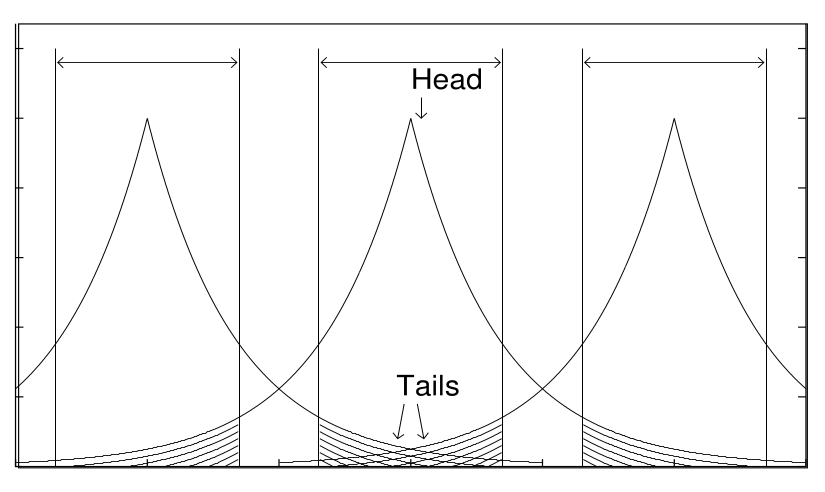
\includegraphics[height=2.55in,width=3.15in,viewport=0 0 845 635,clip]{Figures/MTO-Tail_cancellation.png}
\caption{\small \textrm{The wavefunction in the spere at the origin is the sum of the ``head function'' in that sphere plus the tails from neighboring spheres. The schematic illustration of the ``tail cancellation'' of the MTO.}}%(与文献\cite{EPJB33-47_2003}图1对比)
\label{MTO-tail-candellation}
\end{figure}
}

\frame
{
	\frametitle{\textrm{LMTO}方法}
	与\textrm{LAPW}方法类似,在给定能量$\varepsilon_v$和衰减常数$q_0$附近,\textrm{LMTO}的基函数球内部分用函数$\psi(\varepsilon_v,r)$及其对能量导数$\dot\psi(\varepsilon_v,r)$表示\\
\textcolor{blue}{\textrm{LMTO}与\textrm{MTO}基函数的区别}
	\begin{itemize}
		\item 球内部分的$\psi(\varepsilon,r)$是主要部分:~由$\psi(\varepsilon_v,r)$和$\dot\psi(\varepsilon_v,r)$线性组合
		\item 球内来自其它\textrm{MT}球的函数尾部贡献被$\dot\psi(\varepsilon_v,r)$的线性组合替代
	\end{itemize}
	由此根据物理直觉,可以把\textrm{LMTO}基函数的形式表示成
		\begin{displaymath}
			\hspace*{-12pt}\chi_L^{\mathrm{LMTO}}(\varepsilon,q_0,\vec r)=\mathrm{i}^lY_L(\hat{\vec r})\left\{
			\begin{aligned}
				&\psi_l(\varepsilon,r)-q_0\cot(\eta_l(\varepsilon))J_l(q_0r)&\, r\leqslant S\\
				&q_0N_l(q_0r)&\, r>S
			\end{aligned}\right.
		\end{displaymath}
		实际应用中,选定函数$J_l$和$N_l$与球\textrm{Bessel}函数$j_l$和\textrm{Neumann}函数$n_l$相似
}

\frame
{
	\frametitle{\textrm{LMTO}方法}
	根据物理边界要求,在\textrm{MT}球内,基函数$\chi_L^{\mathrm{LMTO}}$对能量$\varepsilon$的导数在$\varepsilon=\varepsilon_v$为0可确定$J_l$
		\begin{displaymath}
				J_l(q_0r)=-\dfrac{\dot\psi_l(\varepsilon_v,r)}{q_0\frac{\mathrm{d}}{\mathrm{d}\varepsilon}\cot(\eta_l(\varepsilon_v))},\,r\leqslant S
		\end{displaymath}
		$N_L$的定义与\textrm{Neumann}函数相似,在极限条件$n_l\rightarrow N_l$,$j_l\rightarrow J_l$,其它\textrm{MT}球的函数尾巴满足多重散射展开方式
		\begin{displaymath}
				N_L(q_0,\vec r-\vec R)=4\pi\sum_{L^{\prime},L^{\prime\prime}}C_{L^{\prime}L^{\prime\prime}}^Ln_{L^{\prime\prime}}^{\ast}(q_0,\vec R-\vec R\,^{\prime})J_{L^{\prime}}(q_0,\vec r-\vec R\,^{\prime}),\,r>S
		\end{displaymath}
		由此得到的能量无关的\textrm{LMTO}基函数满足
		\begin{itemize}
			\item \textcolor{blue}{在\textrm{MT}球内函数由$\psi$和$\dot\psi$的线性组合}
			\item \textcolor{blue}{\textrm{MT}球内函数光滑延伸到\textrm{MT}外,并能与其余\textrm{MT}球函数能量导数$\dot\psi$光滑连续}
		\end{itemize}
}

\frame
{
	\frametitle{\textrm{LMTO}方法}
	对于周期体系,取$q_0=0$~,\textrm{LMTO}方法的基函数可以表示为
	\begin{displaymath}
		\chi_{L,\vec k}^{\mathrm{LMTO}}(\vec r)=\dfrac{\psi_{L-}(\vec r)}{\psi_{l-}(S)}-\dfrac1{\psi_{l+}(S)}\sum_{L^{\prime}}\psi_{L^{\prime}+}(\vec r)\dfrac1{2(2l^{\prime}+1)}S_{LL^{\prime}}(\vec k)
	\end{displaymath}
	这里$\psi_{l-}(r)\equiv\psi_l(D=-l-1,r)$,$(r/S)^l\rightarrow\psi_{l+}(r)\equiv\psi_l(D=l,\varepsilon)$
	$$\psi(D,r)=\psi(r)+\omega(D)\dot\psi(r)$$
	这里
	$$\omega(D)=-\dfrac{\psi(S)D-D(\psi)}{\dot\psi(S)D-D(\dot\psi)}$$
	这里$D(\psi)$和$D(\dot\psi)$分别是$\psi$和$\dot\psi$的对数导数

	由此定义的\textrm{LMTO}基函数
	\begin{itemize}
		\item \textcolor{red}{对能量$\varepsilon_v$依赖到一阶}
		\item \textcolor{red}{径向函数在\textrm{MT}球外的尾巴抵消保持到计算所需要的最低阶}
	\end{itemize}
}

\frame
{
	\frametitle{\textrm{LMTO}方法}
	\textcolor{blue}{\textrm{KKR}、\textrm{MTO}、\textrm{LMTO}方法的特点}
	\begin{enumerate}
   		\setlength{\itemsep}{15pt}
		\item \textcolor{red}{\textrm{KKR}方法的基函数选择对计算结果影响较大}
		\item \textcolor{red}{\textrm{KKR}方法的基函数适应范围广}:\\可以方便地应用到局域体系、周期体系和掺杂(或合金)体系
		\item \textcolor{red}{\textrm{MTO}和\textrm{LMTO}构造的基函数是优化最小基组}:~计算效率高
		\item \textcolor{red}{\textrm{MTO}和\textrm{LMTO}的基函数构造比较复杂}
	\end{enumerate}
}


\appendix
%------------------------------------------------------------------------Reference----------------------------------------------------------------------------------------------
%\begin{thebibliography}{99}
%-----------------------------------------------------------------------------------------------------------------------------------------------------------------------%
%\frame
%{
%\frametitle{主要参考文献}
%{\small
%\bibitem{Singh_Book}\textrm{D. J. Singh. \textit{Plane Wave, PseudoPotential and the LAPW method} (Kluwer Academic, Boston,USA, 1994)}					%
%  \nocite{*}																				%
%}
%}
%\end{thebibliography}
\begin{thebibliography}{99}
\frame
{
\frametitle{主要参考文献}
{\small
%	\bibitem{Huang_Han}黄昆\:原著、韩汝琦\:改编, {\textit{固体物理学}}\:高等教育出版社, 北京, 1988
%	\bibitem{Xie_Lu}谢希德、陆栋\:主编, {\textit{固体能带理论}}\:复旦大学出版社, 上海, 1998
	\bibitem{PA13-392_1947}\textrm{J. Korringa. \textit{Physica}, \textbf{13} (1947), 392}
	\bibitem{PR94-1111_1954}\textrm{W. Kohn and N. Rostocker. \textit{Phys. Rev.} \textbf{94} (1954), 1111}
%	\bibitem{SSC114-15_2000}\textrm{E. Sj\"ostedt, L. Nordstr\"om and D. J. Singh. \textit{Solid State Commun.}, \textbf{114} (2000), 15}
	\bibitem{Comp_Method}\textrm{V. V. Nemoshkalenko and V. N. Antonov. \textit{Computational Methods in Solid State Physics} (Gordon and Breach Science Publisher, Amsterdam, The Netherlands, 1998)}
	\bibitem{JPCM14-2799_2002}\textrm{N. Papanikolaou, R. Zeller and P. H. Dederichs. \textit{J. Phys.: Condens. Matter.} \textbf{14} (2002), 2799}
	\bibitem{Andersen_Book}\textrm{O. K. Andersen. \textit{Computational Methods in Band Theory} (Plenum, New York, USA, 1971)}
	\bibitem{LMTO_Book}\textrm{H. Skriver. \textit{The LMTO method} (Springer, New York, USA, 1984)}
	\bibitem{PRB12-3060_1975}\textrm{O. K. Andersen. \textit{Phys. Rev.} B, \textbf{12} (1971), 3060}
	\bibitem{Elect_Stru}\textrm{Richard. M. Martin. \textit{Electronic Structure: Basic Theory and Practical Methods} (Cambridge University Press, Cambridge, England, 2004)}
%        \bibitem{Singh_Book}\textrm{D. J. Singh. \textit{Plane Wave, PseudoPotential and the LAPW method} (Kluwer Academic, Boston,USA, 1994)}
}
\nocite*{}
}
\end{thebibliography}
%{\small
%\phantomsection\addcontentsline{toc}{section}{Bibliography}	 %直接调用\addcontentsline命令可能导致超链指向不准确,一般需要在之前调用一次\phantomsection命令加以修正	%
%\bibliography{Myref}																			%
%\bibliographystyle{mybib}																		%
%  \nocite{*}																				%
%}
%-----------------------------------------------------------------------------------------------------------------------------------------------------------------------%


%-----------------------------------------------------------Beamer下不建议使用bib,因为涉及分页--------------------------------------------------------------------------%
%{\small
%\phantomsection\addcontentsline{toc}{section}{Bibliography}	 %直接调用\addcontentsline命令可能导致超链指向不准确,一般需要在之前调用一次\phantomsection命令加以修正	%
%\bibliography{Myref}																			%
%\bibliographystyle{mybib}																		%
%  \nocite{*}																				%
%}

%------------------------------------------------------------------------------------------------------------------------------------------------------------------------------%

%-------------------------------------------------------------------------Thanks------------------------------------------------------------------------------------------------
%\section{致谢}
%\frame
%{
%\frametitle{致$\quad$谢}
%\begin{itemize}
%    \setlength{\itemsep}{20pt}
%  \item 感谢本团队高兴誉、吴泉生、宋红州等各位老师参与的讨论
%  \item 感谢莫所长、宋主任以及软件中心各位老师和同事
%  \item 感谢王崇愚先生的帮助
%\end{itemize}
%}

\logo{}									%不显示logo
\frame
{
\vskip 60 pt
%\hskip 10pt \textcolor{blue}{\Huge 感谢答辩委员会各位老师\,\textrm{!}}\\
\vskip 35 pt
\hskip 60pt \textcolor{blue}{\Huge 谢谢大家\:!}
%\vskip 15 pt
%\hskip 40pt \textcolor{blue}{\Huge \textrm{for your attention\:!}}
}

%-------------------------------------------------------------------------------------------------------------------------------------------------------------------------------

\clearpage
%\end{CJK*}
\end{document}
